\chapter{附录：补充图表、实验细节与扩展讨论}

\section{数据集与实验任务补充说明}
为了使全文的实验设置更加清晰，本附录对各章涉及的数据集、迁移任务以及评价方式进行统一补充。核检测与核实例分割部分主要围绕 CoNSeP、MoNuSAC、Lizard、PanNuke 以及肾透明细胞癌相关病理数据展开。这些数据集在组织来源、染色风格、目标类别定义和实例密度上均存在明显差异，因此非常适合用于验证模型的跨域能力与未见类别泛化能力。

在第三章和第五章的实验中，任务通常具有 few-shot 或 prompt-based 适配特征，即源域模型首先在完整训练集上学习通用表示，再通过目标域少量支持图像或提示信息完成适配。第四章则更强调零样本检测与自训练，目标是在不依赖目标域检测标注的条件下，通过视觉语言先验和自动属性提示建立可用的初始检测能力。第六章的数字病理分析工作则不再以 benchmark 风格任务为主，而是更关注识别结果如何被转化为临床相关的量化指标。

\section{评价指标补充说明}
全文使用的评价指标具有多层含义。对于核实例分割任务，Dice、AJI、对象级 Dice、PQ 与 F1 共同构成了一个较全面的评价体系。其中 Dice 更强调整体前景重叠程度，AJI 强调实例级聚合质量，对象级 Dice 强调匹配实例后的平均重叠程度，PQ 则综合考虑检测质量与分割质量。对于检测任务，AP 与 AR 分别从精度和召回两个角度评价模型表现。对于临床应用章节，重点则转向病理一致性分析、组间比较与生存分析。

在毕业论文写作中，补充这些指标的概念与适用场景尤为重要，因为不同章节的研究目标并不完全相同。若不说明指标差异，读者容易误以为全文所有实验都在追求同一类分数。实际上，第三章和第五章更强调实例结构恢复，第四章更强调检测入口建立，第六章则强调下游临床解释性。

\section{实现细节与复现流程补充}
本论文涉及的模型实现横跨弱监督实例分割、零样本检测、视觉文本化和数字病理分析多个方向，因此复现流程需要额外说明。总体上，作者采用统一的视觉语言预训练框架作为骨架，并在此基础上逐步扩展不同任务所需的提示学习、结构解耦与适配模块。对于需要支持图像的实验，通常要先在源域完成模型预训练，再在目标域利用少量支持样本构造提示表示；对于零样本检测实验，则需要先完成属性提示构造，再利用零样本输出作为伪标签执行自训练。

此外，跨域实验中的数据集映射与 few-shot 抽样策略对结果影响很大。为了保证实验公平性，作者在不同方法间尽量使用同一批目标域支持图像，并通过固定随机种子生成用于统计标准差的多个实验重复。对于大论文而言，这类工程规范虽然不一定直接提升结果分数，但却决定了整套实验结论是否具有可解释性和可信度。

\section{第三章补充图表与讨论}
\begin{figure}[H]
  \centering
  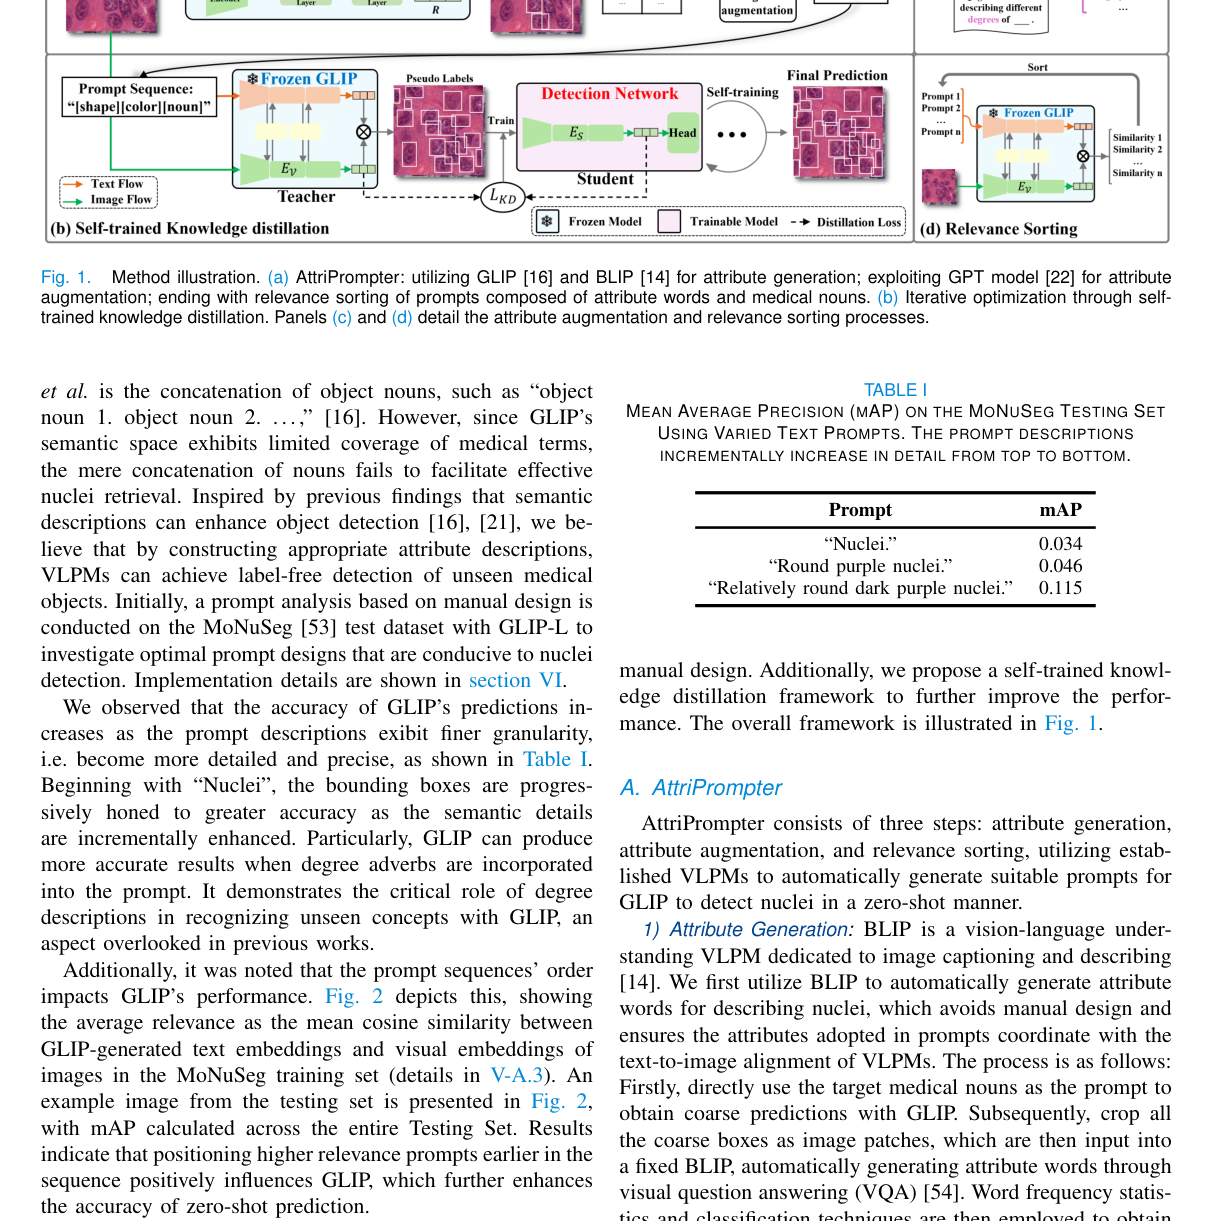
\includegraphics[width=0.92\textwidth]{figures/tmi_fig_method.png}
  \caption{第三章工作的补充框架图。该图以论文原始英文图为基础，在学位论文中可直接配合中文图题使用。}
\end{figure}

\begin{figure}[H]
  \centering
  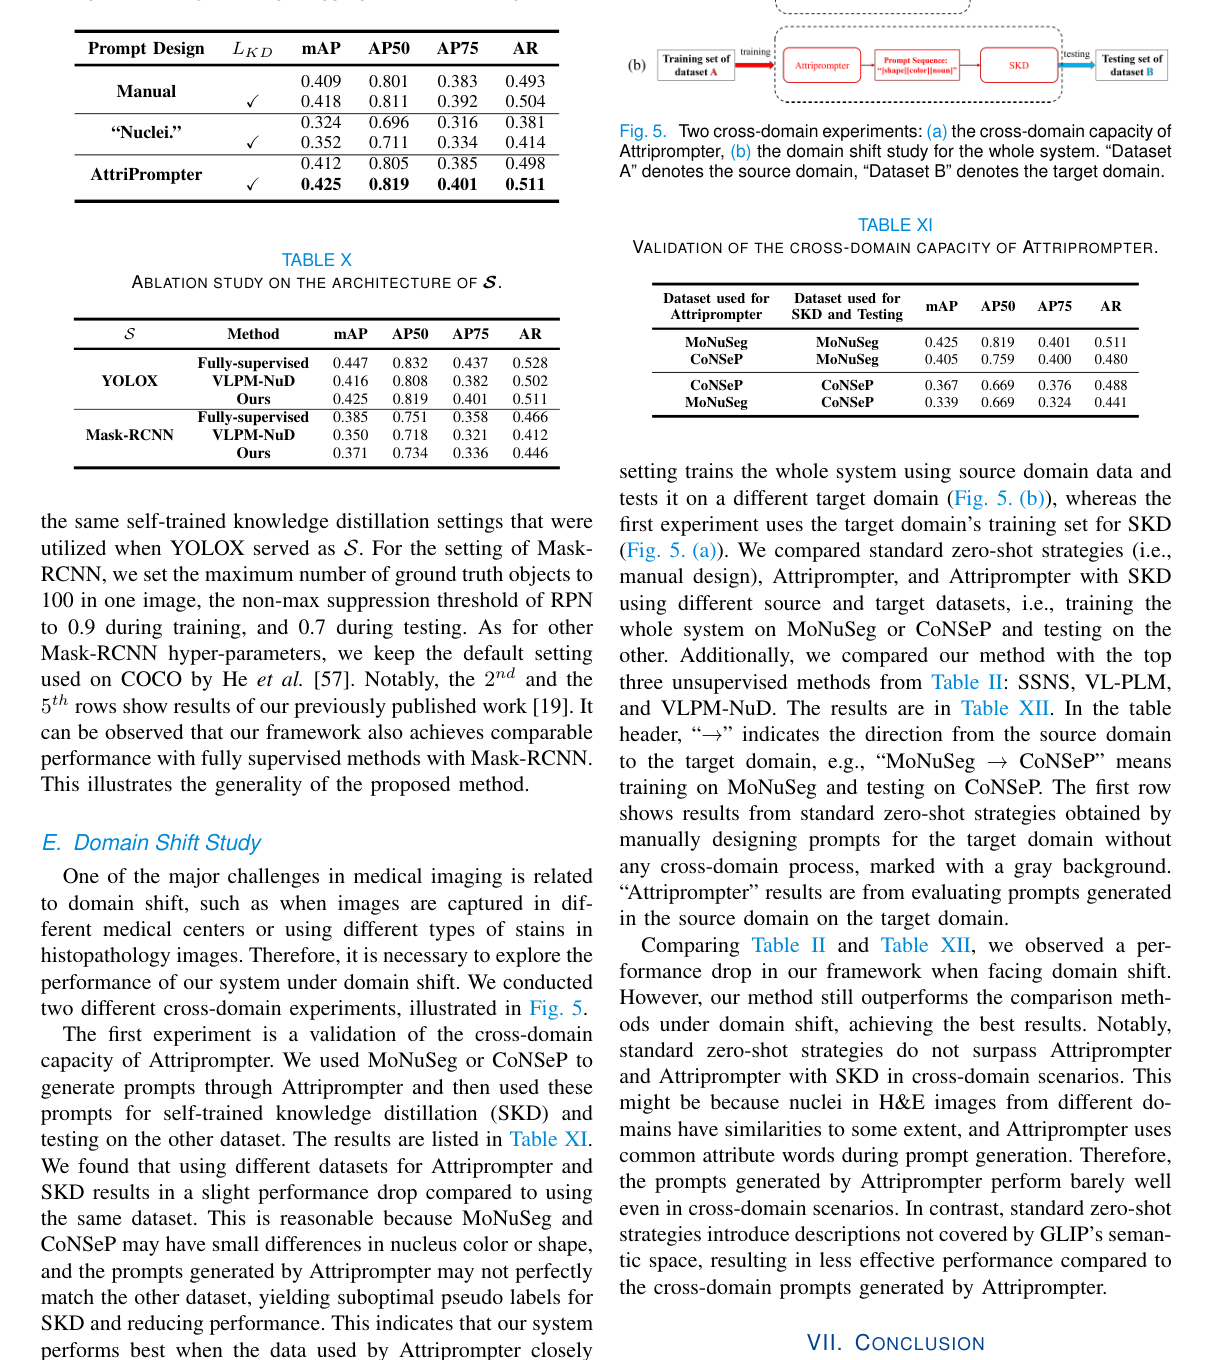
\includegraphics[width=0.92\textwidth]{figures/tmi_table_more_ablation.png}
  \caption{第三章工作的补充消融结果。通过增加该图，可以更充分地支撑属性解耦提示机制的有效性分析。}
\end{figure}

这些补充图表在学位论文中的作用不仅是“增加页数”，更重要的是让章节叙述与原始论文证据链形成紧密对应。特别是在答辩或导师审阅场景中，图表与正文一一对应，可以帮助读者快速理解该章的关键贡献点和实验支撑关系。

\section{第四章补充图表与讨论}
\begin{figure}[H]
  \centering
  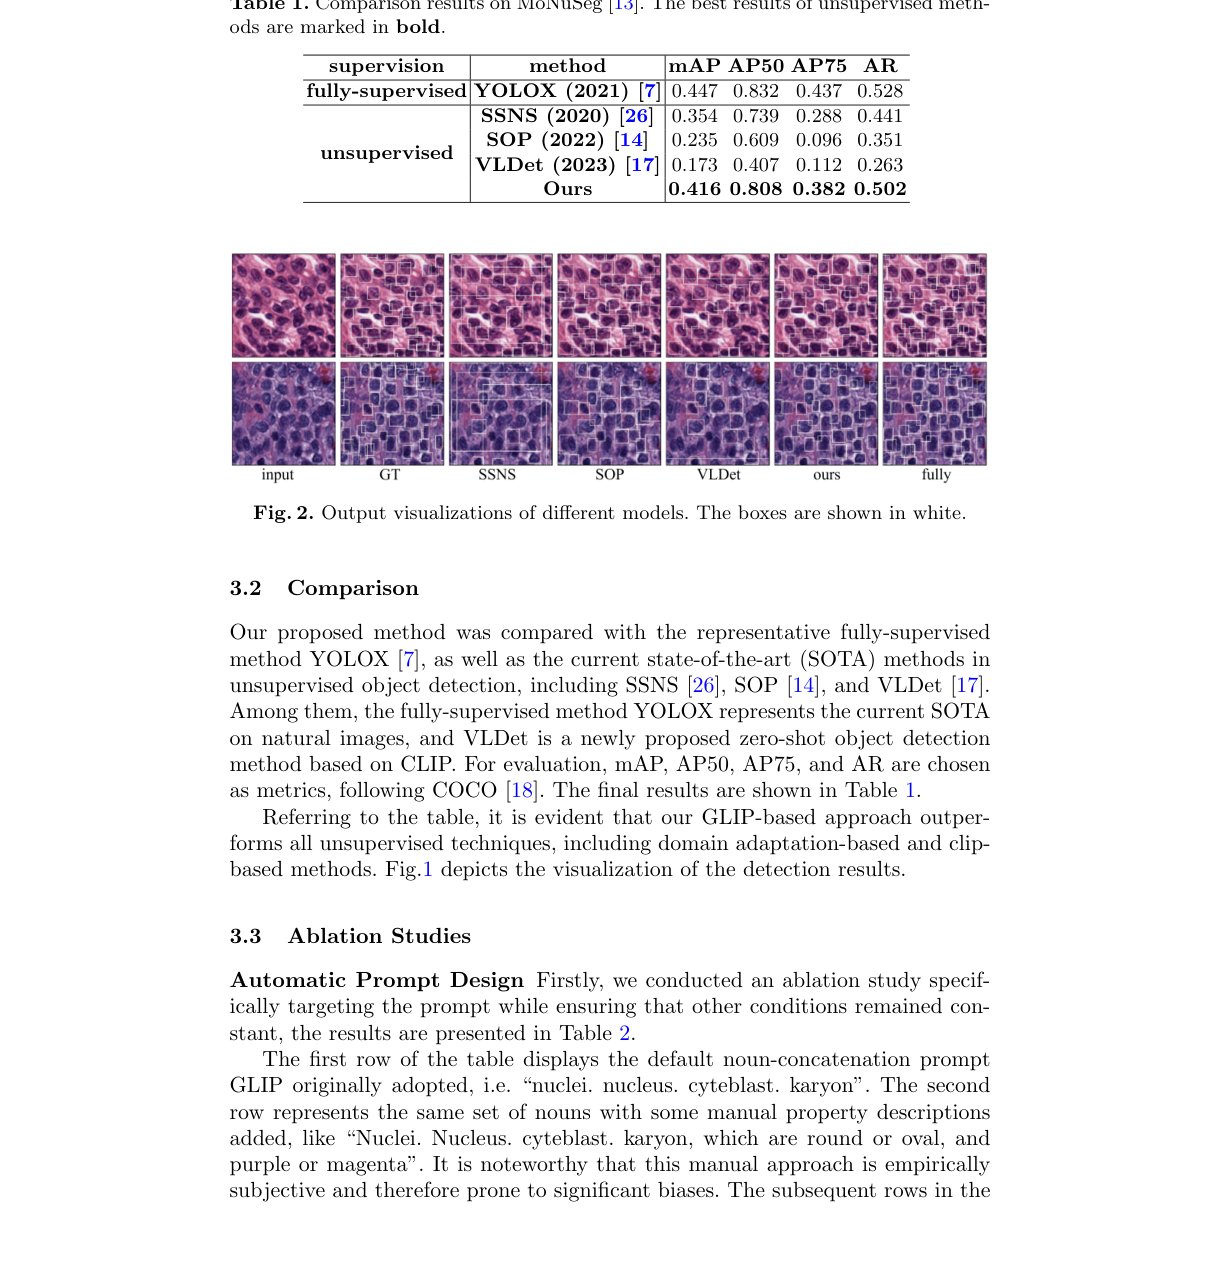
\includegraphics[width=0.9\textwidth]{figures/miccai_table_main.png}
  \caption{第四章主要检测结果补充图。由于原始论文以英文表格呈现，这里保留原图并辅以中文叙述，可较快扩充大论文章节内容。}
\end{figure}

\begin{figure}[H]
  \centering
  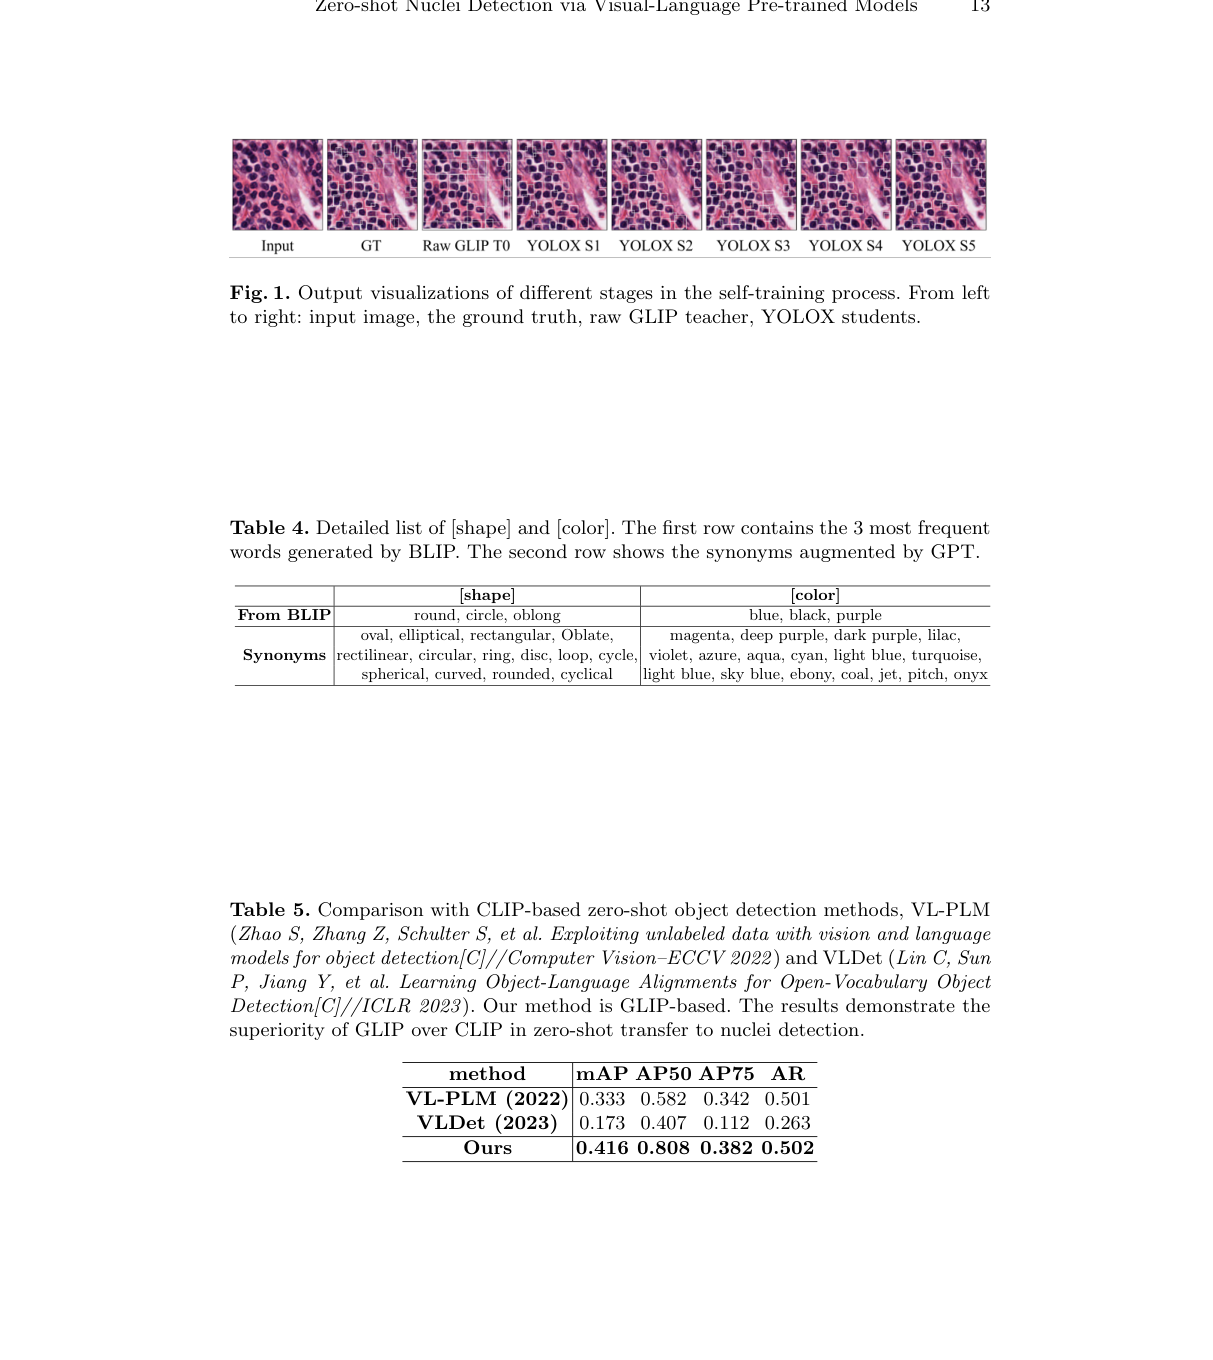
\includegraphics[width=0.9\textwidth]{figures/miccai_fig_selftrain.png}
  \caption{第四章自训练增益补充图。该图适合与正文中的“从零样本预测到目标域适配”的叙述相配合。}
\end{figure}

与第三章类似，第四章的补充图表强化了“自动属性提示 + 自训练”的双阶段逻辑。把这类图表单独置于附录，一方面可以避免主体章节过于拥挤，另一方面也能在审稿或送审版本中体现工作量与证据链的完整性。

\section{第五章补充图表与讨论}
\begin{figure}[H]
  \centering
  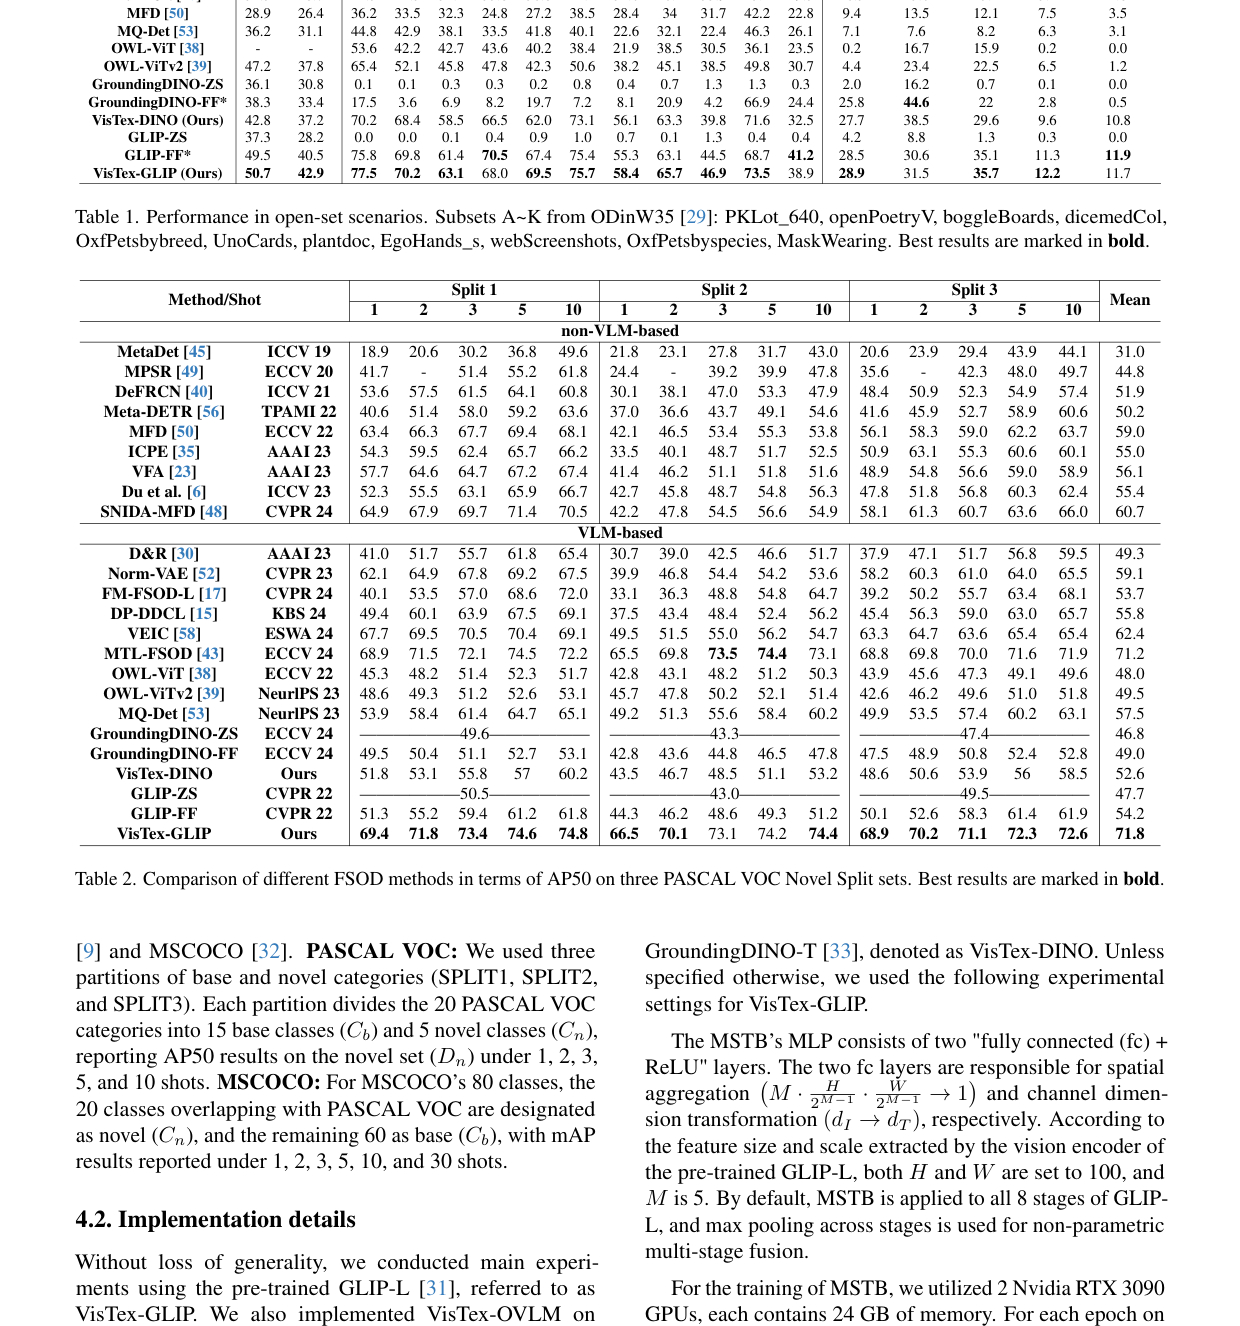
\includegraphics[width=\textwidth]{figures/vistex_table_main.png}
  \caption{第五章主要结果补充图。该图展示 VisTex 与多种基线方法在跨域提示任务中的总体比较。}
\end{figure}

\begin{figure}[H]
  \centering
  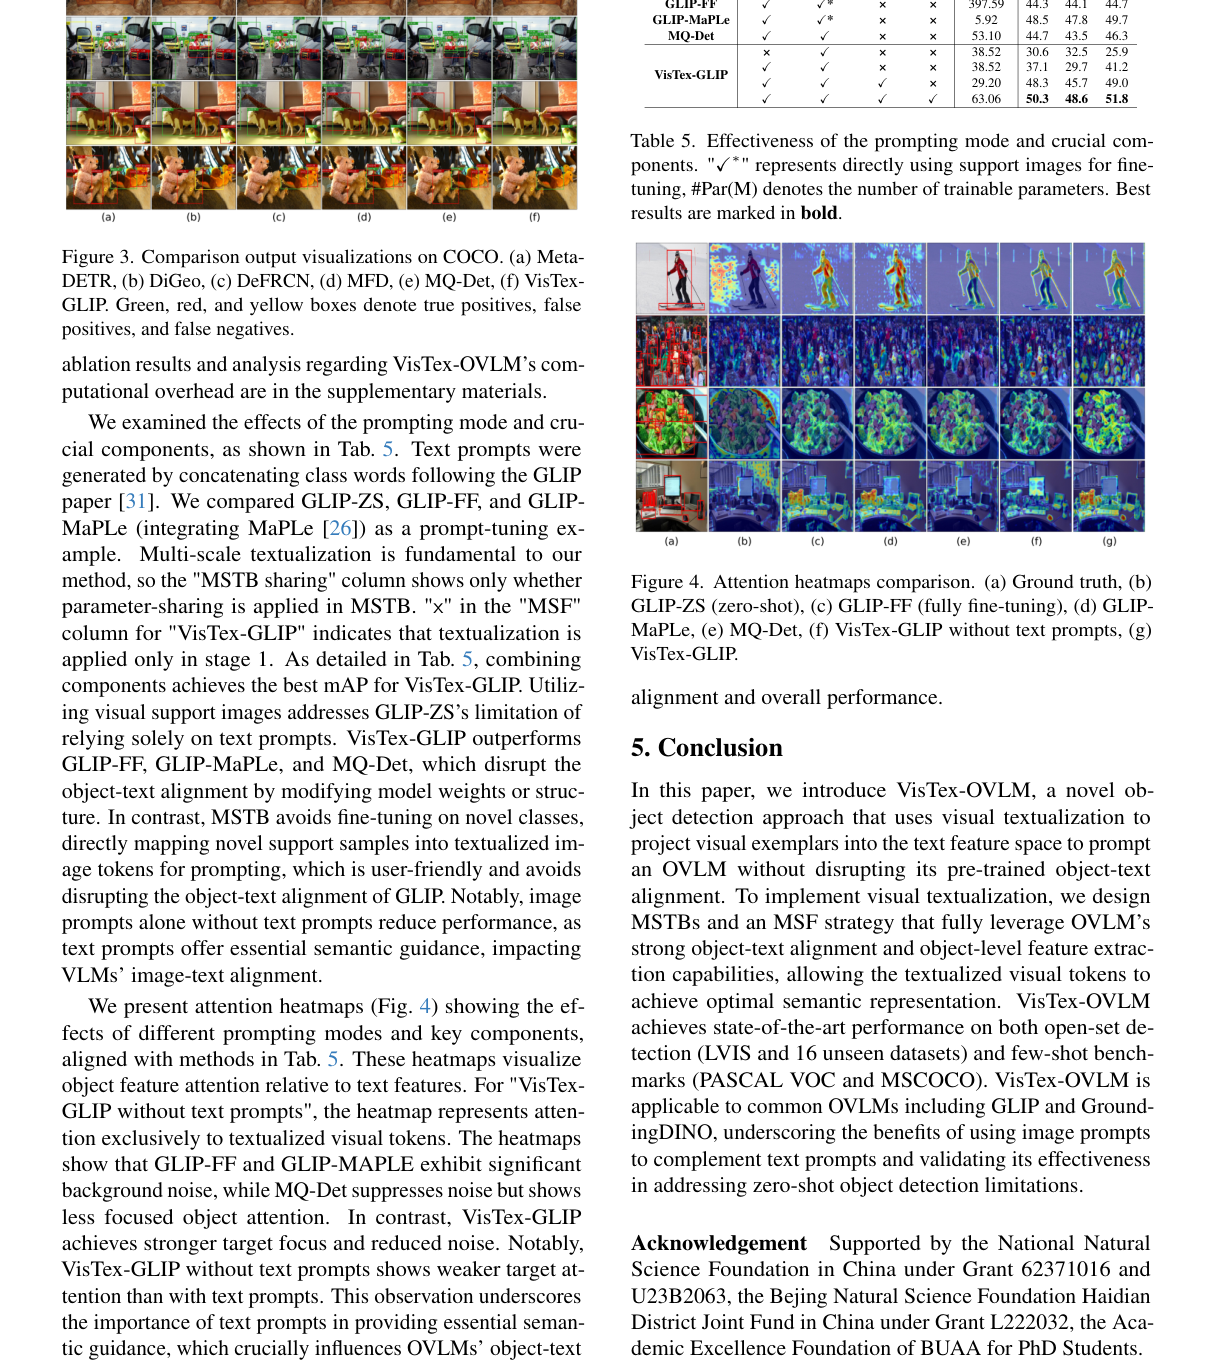
\includegraphics[width=\textwidth]{figures/vistex_fig_vis.png}
  \caption{第五章可视化案例补充图。该图有助于展示图像提示对困难样本的具体改善方式。}
\end{figure}

在大论文写作中，第五章往往最容易因为方法较新、概念较多而显得抽象。通过增加框架图、主结果表和可视化对比图，可以显著提升章节的可读性，使读者更容易理解“视觉文本化”究竟带来了什么。

\section{第六章补充图表与讨论}
\begin{figure}[H]
  \centering
  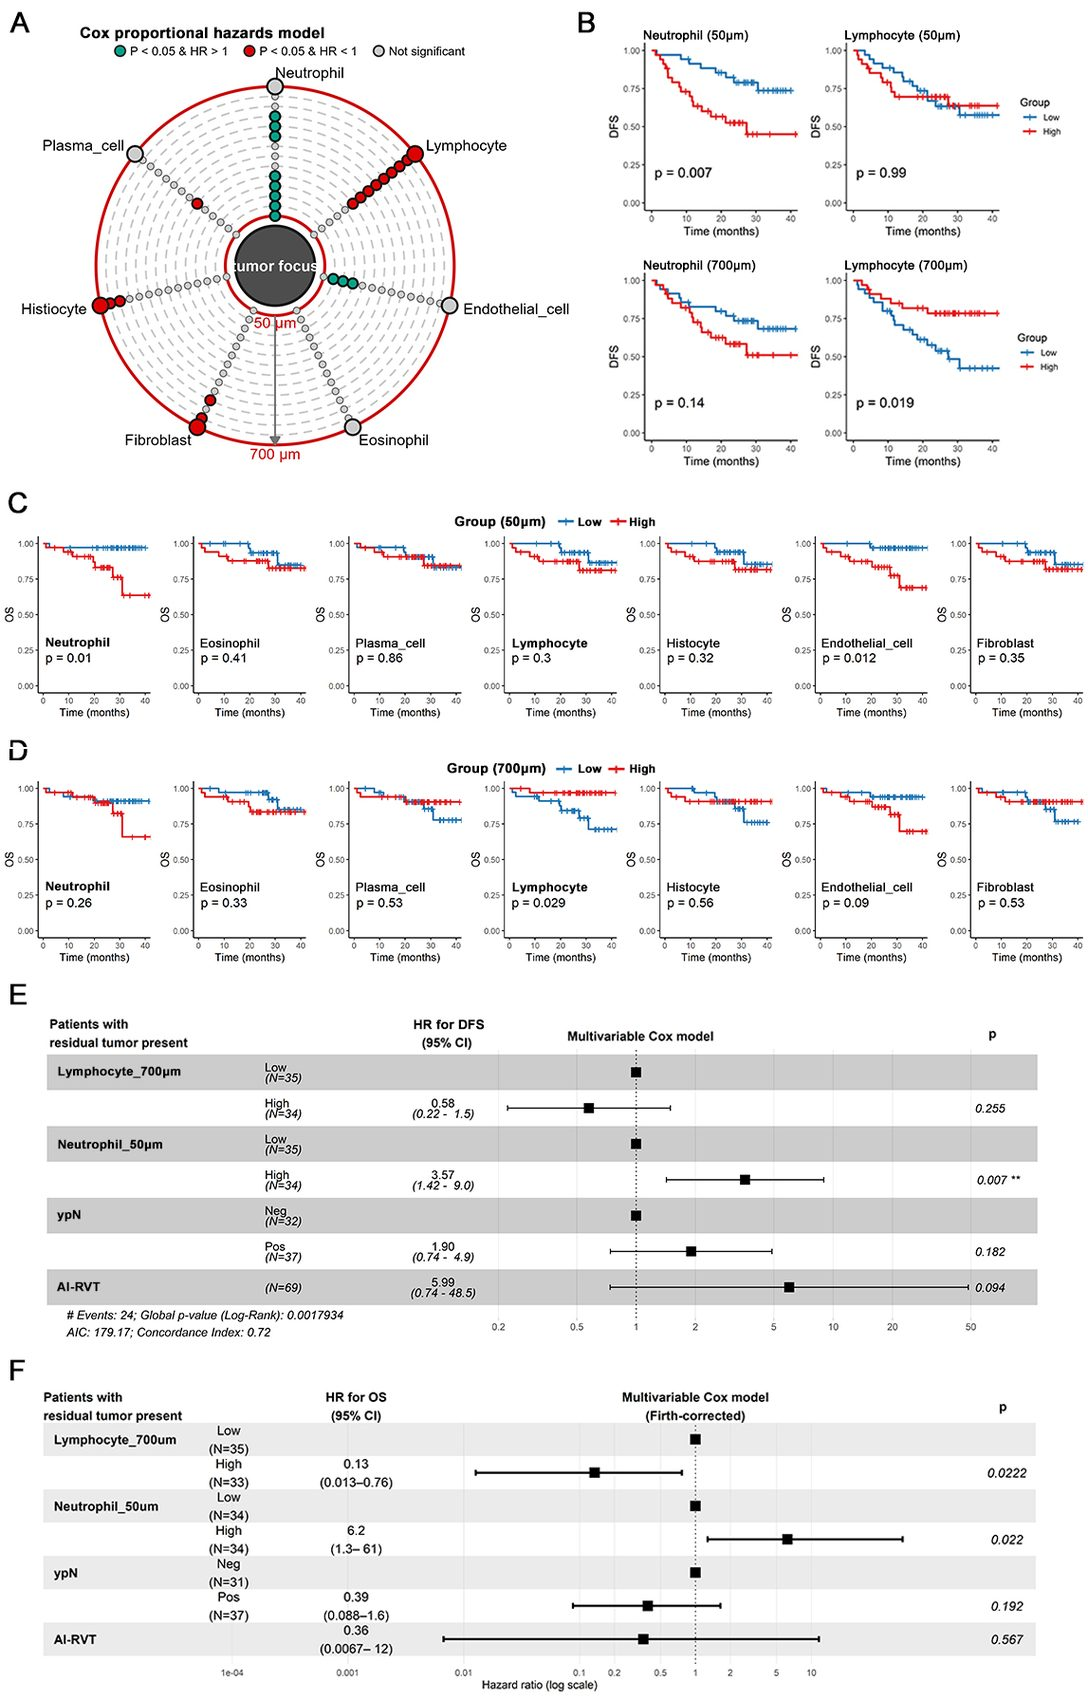
\includegraphics[width=\textwidth]{figures/lung_image5.jpeg}
  \caption{第六章生存分析补充图。将该类图表纳入学位论文附录，有助于增强临床分析部分的完整性。}
\end{figure}

\begin{figure}[H]
  \centering
  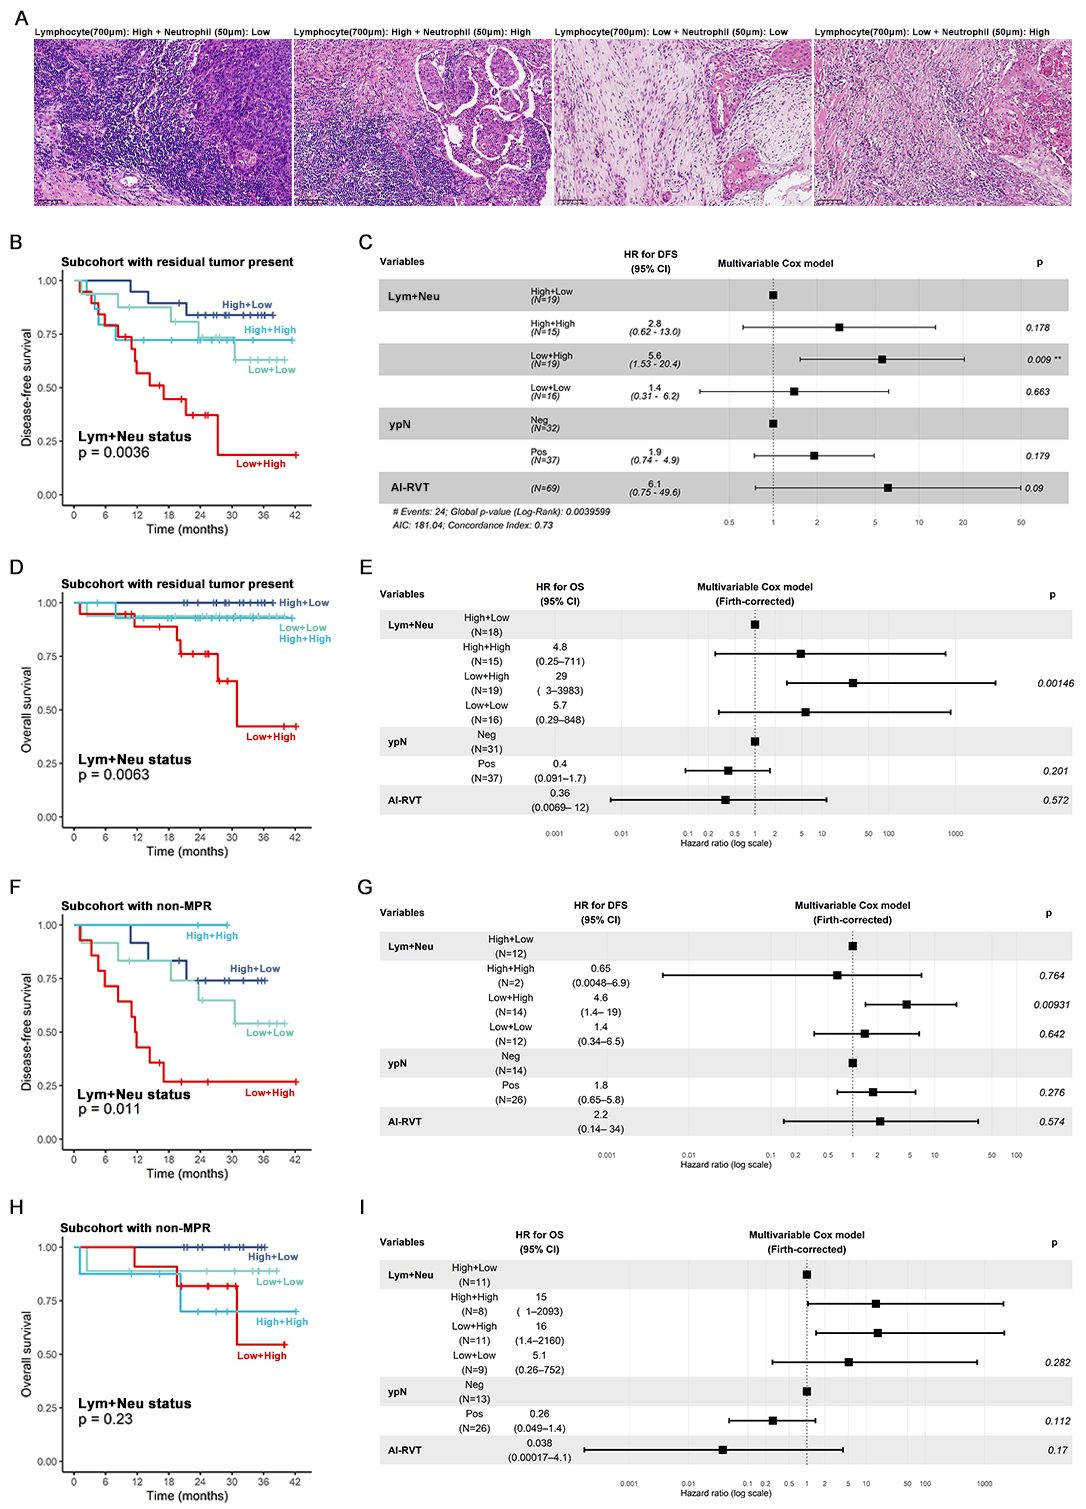
\includegraphics[width=\textwidth]{figures/lung_image6.jpeg}
  \caption{第六章亚组分析补充图。该图可用于说明数字病理指标在不同患者群体中的稳定性。}
\end{figure}

对于临床应用章节而言，图表的作用尤其突出。因为这类工作最终关注的是“指标是否具有临床解释性”，而临床解释性往往必须通过统计图、风险分层图和生存分析图来体现。把这部分材料系统纳入附录，也有助于后续把学位论文版本与在投论文版本进行更高效的互相映照。

\section{扩展讨论：如何把论文进一步扩充为送审版本}
如果后续仍需要把学位论文进一步扩展到更大体量，一个自然方向是把各章实验分析继续细分。例如，第三章可以单独增加“失败案例分析”和“不同属性分支作用的统计汇总”；第四章可以增加“提示模板的语义层次分析”和“自训练伪标签质量变化曲线”；第五章可以补充“直接测试与微调模式差异分析”；第六章则可以进一步增加病例来源、纳排标准、病理阅片流程以及更多临床协变量分析。

另一个适合扩写的部分是对相关工作的系统梳理。事实上，视觉语言预训练、提示学习、零样本检测、医学 few-shot 学习以及数字病理分析本身都已经形成相对成熟的研究脉络。在毕业论文中，把这些脉络系统梳理出来，不仅有助于增加篇幅，更重要的是能够明确本论文各章在整个研究版图中的定位。也就是说，增加附录和图表只是“做厚”的一种方式，而构建更完整的学术叙事则是让论文真正变得扎实的关键。
